
\chapter{Resultados}
\label{cha:resultados}

Aquí se mostrarán los resultados del proyecto \ldots

Como dijo \cite{lin2015microsoft} \ldots

\section{Introducción}
\label{sec:intro-resultados}

\section{Entorno experimental}
\label{sec:desarrollo-resultados}

\subsection{Bases de datos utilizadas}
\label{subsec:bases-datos}

\subsubsection{PETS2006 Dataset}

\begin{figure}[ht]
  \centering
  \begin{subfigure}[b]{0.4\textwidth}
    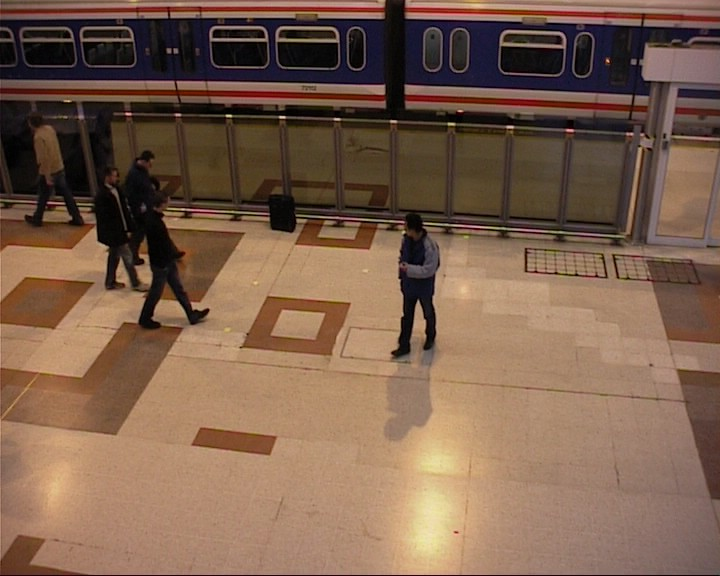
\includegraphics[width=\textwidth]{img/chapters/resultados/bases-datos/pets2006_1.jpeg}
    \caption{}
    \label{fig:pets2006_1}
  \end{subfigure}
  \qquad\qquad
  \begin{subfigure}[b]{0.4\textwidth}
    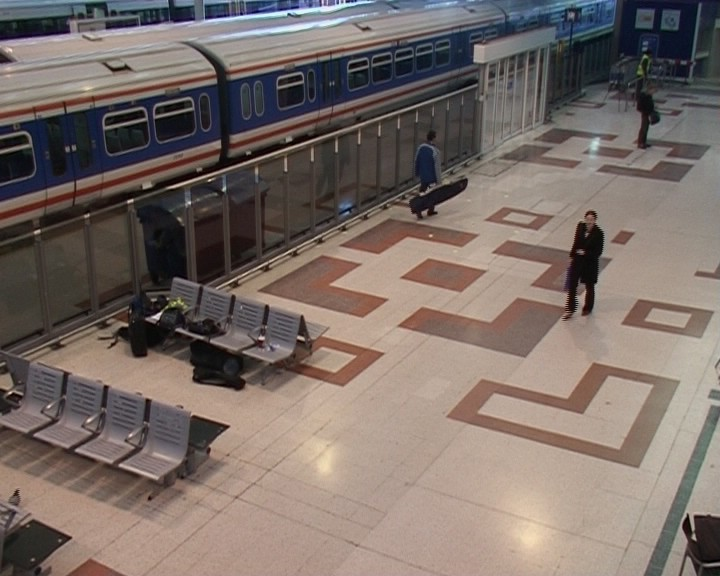
\includegraphics[width=\textwidth]{img/chapters/resultados/bases-datos/pets2006_2.jpeg}
    \caption{}
    \label{fig:pets2006_2}
  \end{subfigure}
  \caption{Imágenes extraídas del dataset PETS2006 \cite{pets2006-dataset}.
    (\protect\subref{fig:pets2006_1}) Frame donde una bolsa de equipaje se encuentra abandonada junto al andén.
    (\protect\subref{fig:pets2006_2}) Otro frame donde varias bolsas y maletas están abandonadas.}
  \label{fig:pets2006}
\end{figure}

\newpage

\subsubsection{PETS2007 Dataset}

\begin{figure}[ht]
  \centering
  \begin{subfigure}[b]{0.4\textwidth}
    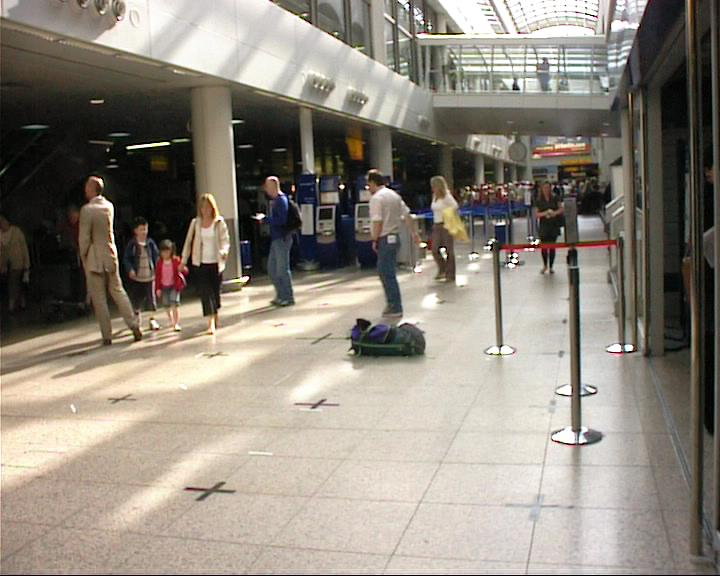
\includegraphics[width=\textwidth]{img/chapters/resultados/bases-datos/pets2007_1.jpeg}
    \caption{}
    \label{fig:pets2007_1}
  \end{subfigure}
  \qquad\qquad
  \begin{subfigure}[b]{0.4\textwidth}
    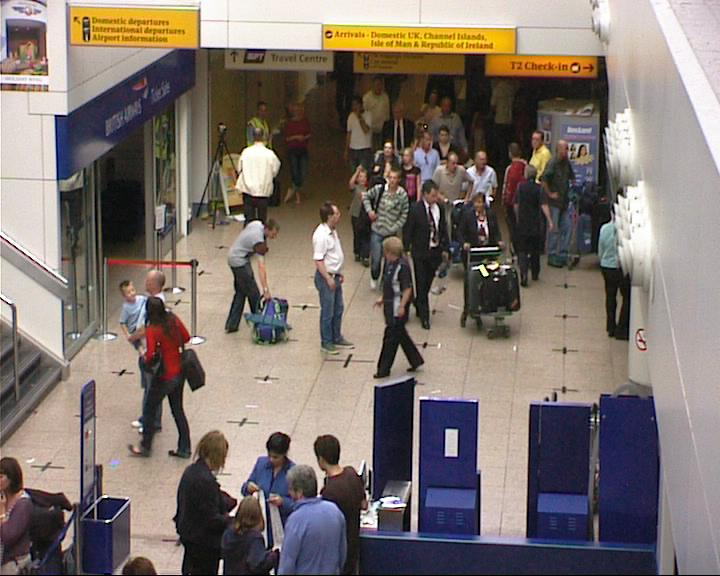
\includegraphics[width=\textwidth]{img/chapters/resultados/bases-datos/pets2007_2.jpeg}
    \caption{}
    \label{fig:pets2007_2}
  \end{subfigure}
  \caption{Imágenes extraídas del dataset PETS2007 \cite{pets2007-dataset}.
    (\protect\subref{fig:pets2007_1}) Frame donde un individuo deja su bolsa de equipaje sobre el suelo.
    (\protect\subref{fig:pets2007_2}) Otro frame en el cual una persona roba el equipaje el individuo.}
  \label{fig:pets2007}
\end{figure}

\subsubsection{AVSS AB 2007 Dataset}

\begin{figure}[ht]
  \centering
  \begin{subfigure}[b]{0.4\textwidth}
    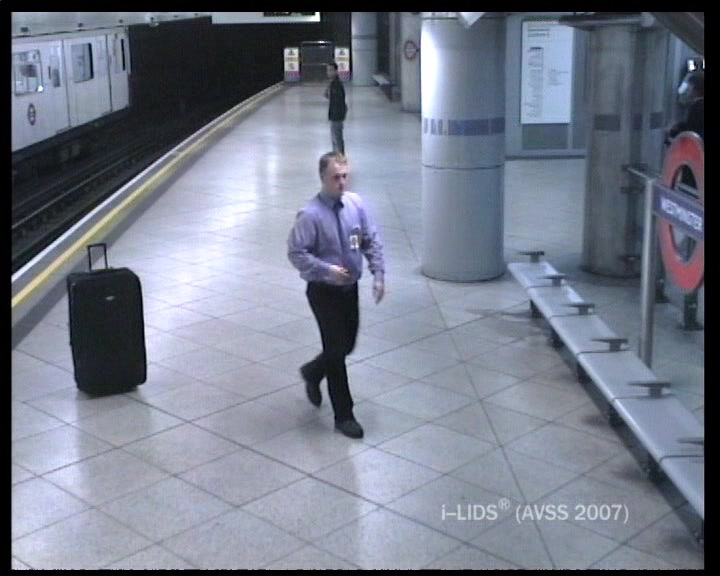
\includegraphics[width=\textwidth]{img/chapters/resultados/bases-datos/AVSSAB_1.jpg}
    \caption{}
    \label{fig:avssab2007_1}
  \end{subfigure}
  \qquad\qquad
  \begin{subfigure}[b]{0.4\textwidth}
    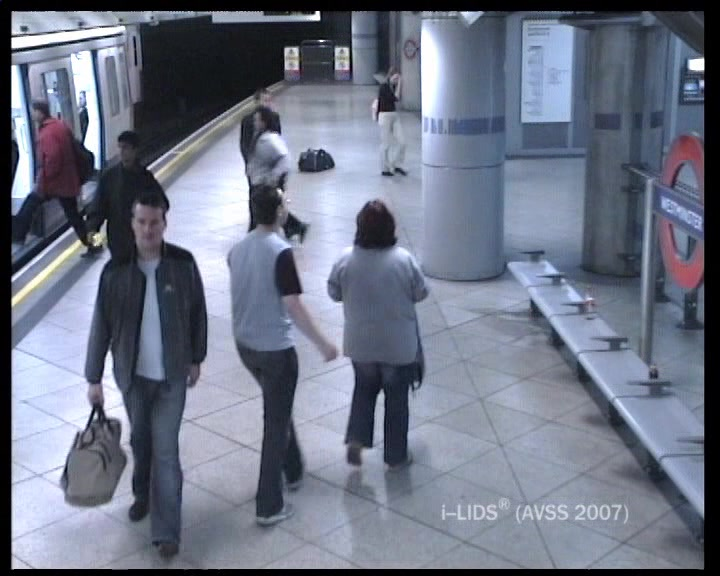
\includegraphics[width=\textwidth]{img/chapters/resultados/bases-datos/AVSSAB_2.jpg}
    \caption{}
    \label{fig:avssab2007_2}
  \end{subfigure}
  \caption{Imágenes extraídas del dataset AVSS AB 2007 \cite{AVSSAB2007-dataset}.
    (\protect\subref{fig:avssab2007_1}) Frame donde un individuo abandona su maleta en el andén.
    (\protect\subref{fig:avssab2007_2}) Otro frame donde una bolsa de equipaje está perdida en el andén durante todo el video.}
  \label{fig:avssab2007}
\end{figure}

\subsubsection{GBA Dataset}

\begin{figure}[ht!]
  \centering
  \begin{subfigure}[b]{0.45\textwidth}
    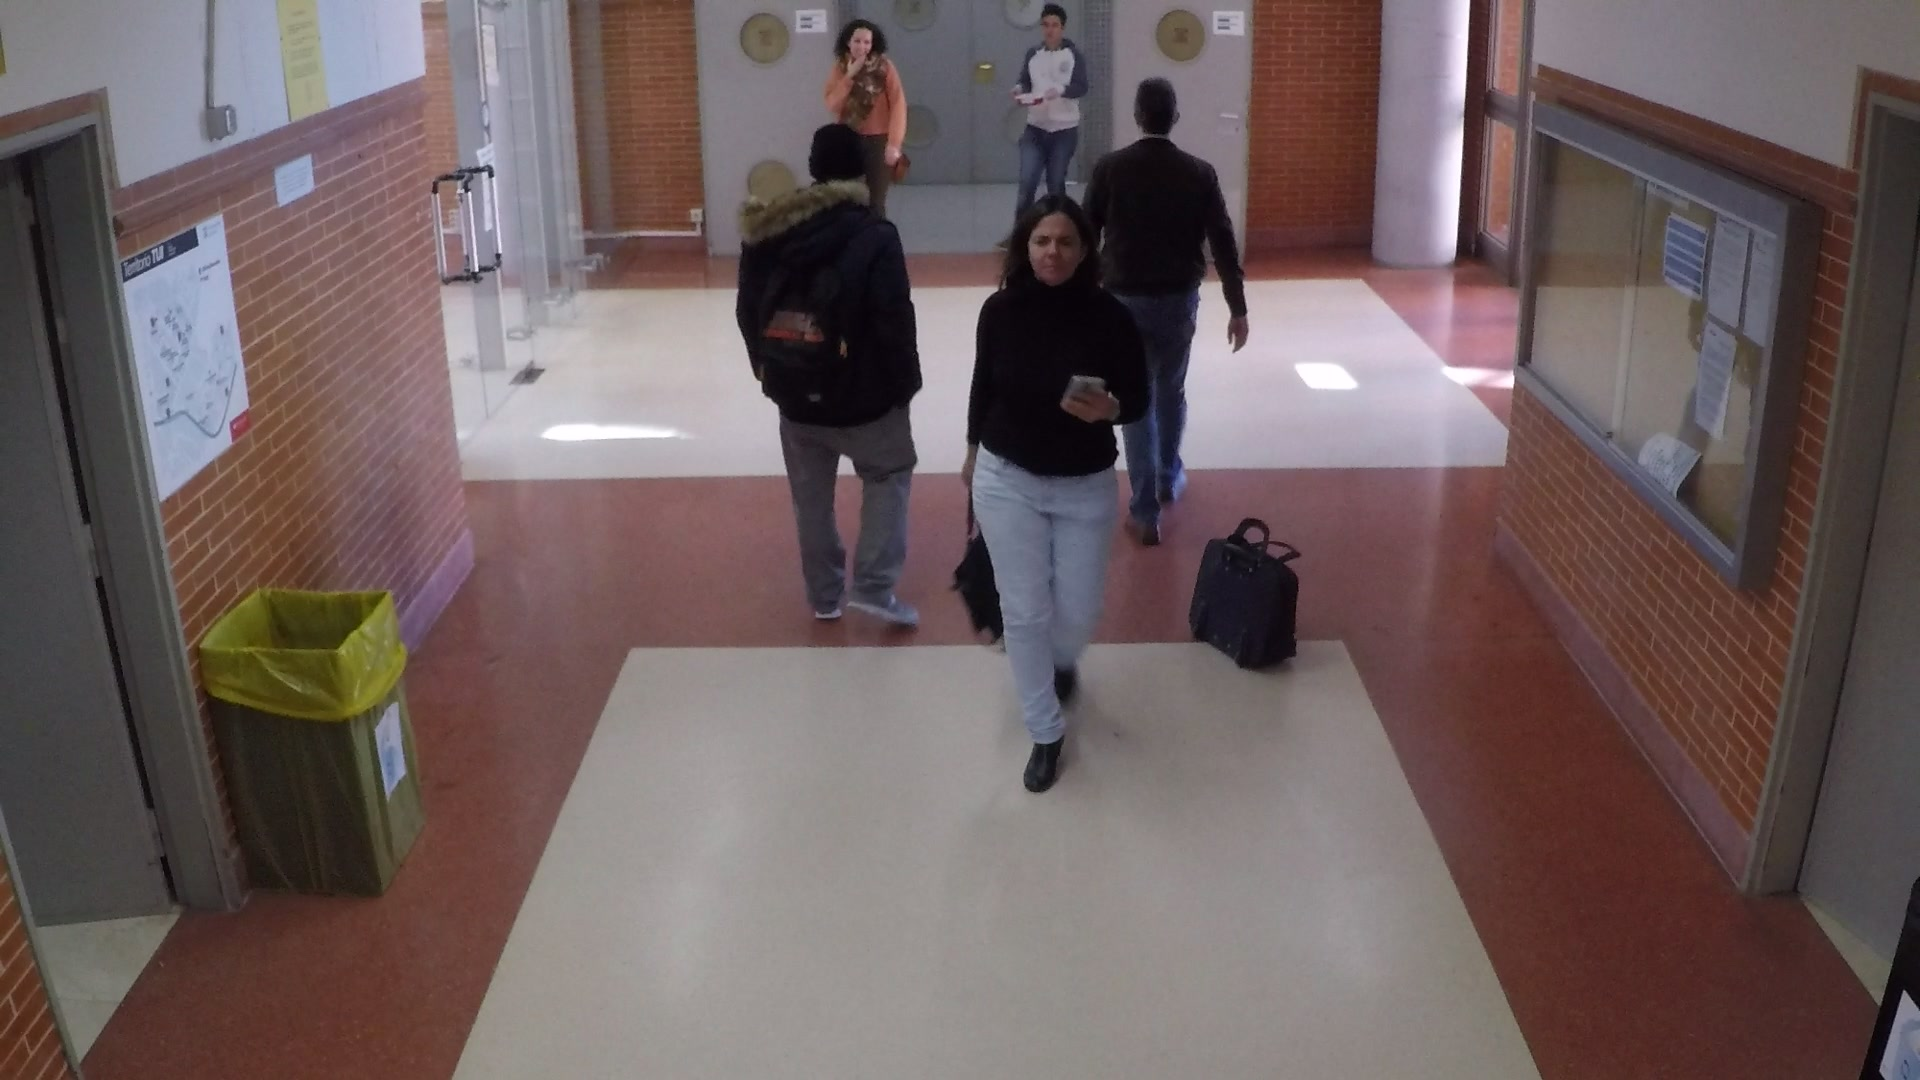
\includegraphics[width=\textwidth]{img/chapters/resultados/bases-datos/GBA_1.jpg}
    \caption{}
    \label{fig:GBA_1}
  \end{subfigure}
  \qquad\qquad
  \begin{subfigure}[b]{0.45\textwidth}
    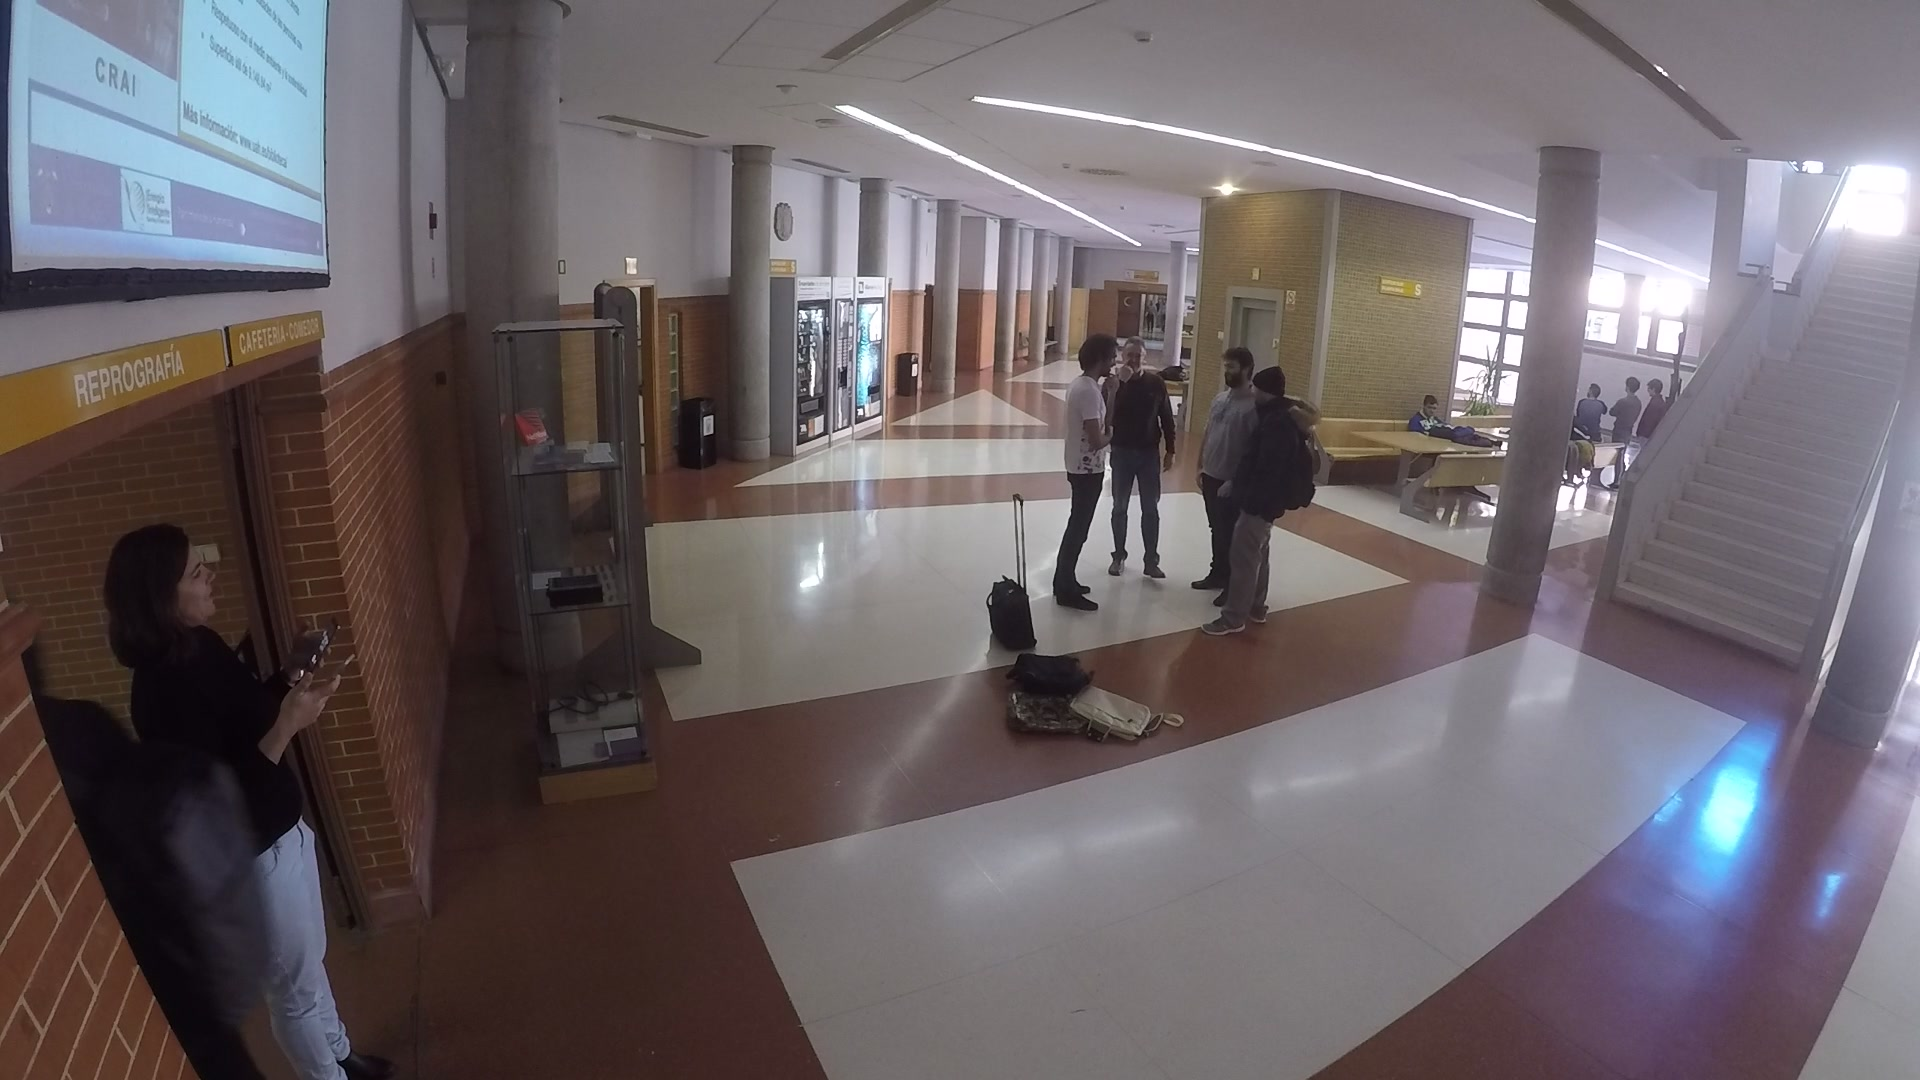
\includegraphics[width=\textwidth]{img/chapters/resultados/bases-datos/GBA_2.jpg}
    \caption{}
    \label{fig:GBA_2}
  \end{subfigure}
  \caption{Imágenes extraídas del dataset GBA \cite{gba-dataset}.
    (\protect\subref{fig:GBA_1}) Frame donde una bolsa de mano es abandonada en el pasillo.
    (\protect\subref{fig:GBA_2}) Otro frame donde varias bolsas y maletas están alejadas de sus propietarios.}
  \label{fig:GBA}
\end{figure}

\subsubsection{AVENUE Dataset}

\begin{figure}[ht]
  \centering
  \begin{subfigure}[b]{0.4\textwidth}
    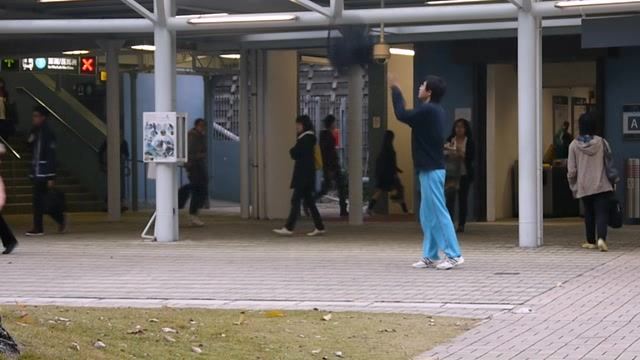
\includegraphics[width=\textwidth]{img/chapters/resultados/bases-datos/avenue_1.jpg}
    \caption{}
    \label{fig:avenue_1}
  \end{subfigure}
  \qquad\qquad
  \begin{subfigure}[b]{0.4\textwidth}
    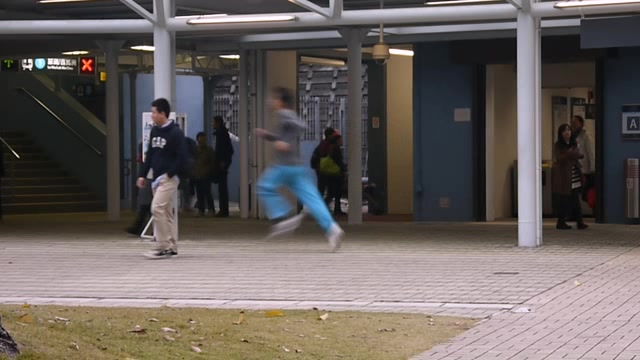
\includegraphics[width=\textwidth]{img/chapters/resultados/bases-datos/avenue_2.jpg}
    \caption{}
    \label{fig:avenue_2}
  \end{subfigure}
  \caption{Imágenes extraídas del dataset AVENUE \cite{avenue-dataset}.
    (\protect\subref{fig:avenue_1}) \textcolor{red}{Frame donde una bolsa de mano es abandonada en el pasillo.}
    (\protect\subref{fig:avenue_2}) \textcolor{red}{Otro frame donde varias bolsas y maletas están alejadas de sus propietarios.}}
  \label{fig:avenue}
\end{figure}

\subsubsection{ABODA Dataset}

\begin{figure}[ht]
  \centering
  \begin{subfigure}[b]{0.4\textwidth}
    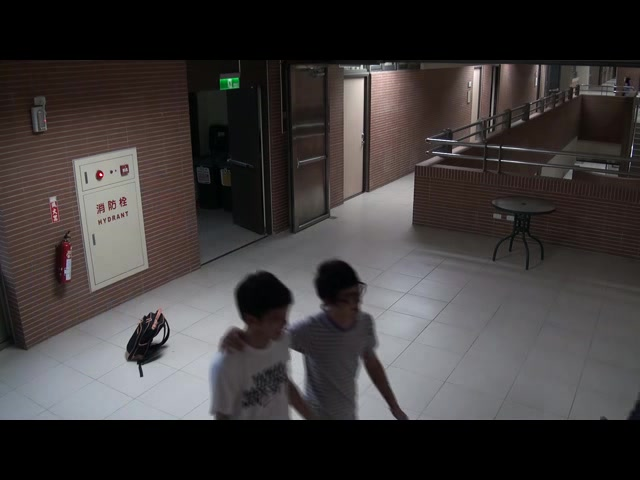
\includegraphics[width=\textwidth]{img/chapters/resultados/bases-datos/aboda_1.jpg}
    \caption{}
    \label{fig:aboda_1}
  \end{subfigure}
  \qquad\qquad
  \begin{subfigure}[b]{0.4\textwidth}
    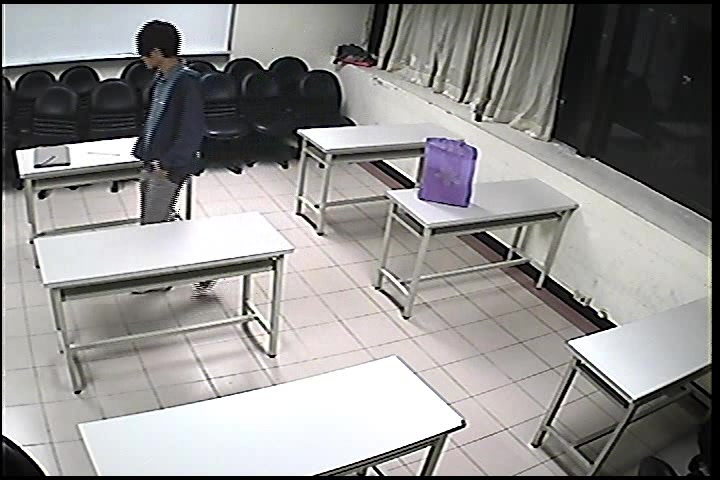
\includegraphics[width=\textwidth]{img/chapters/resultados/bases-datos/aboda_2.jpg}
    \caption{}
    \label{fig:aboda_2}
  \end{subfigure}
  \caption{Imágenes extraídas del dataset ABODA \cite{aboda-dataset}.
    (\protect\subref{fig:aboda_1}) \textcolor{red}{Frame donde una bolsa de mano es abandonada en el pasillo.}
    (\protect\subref{fig:aboda_2}) \textcolor{red}{Otro frame donde varias bolsas y maletas están alejadas de sus propietarios.}}
  \label{fig:aboda}
\end{figure}

\subsubsection{COCO Dataset}

\textcolor{red}{La base de datos COCO es gran conjunto que contiene más de 200 000 imágenes distribuidas en 80 clases de objetos que representan escenas del mundo real. Es una base de datos lo suficientemente grande para que una red bien entrenada con este conjunto de datos sea capaz de aprender características visuales de calidad para el reconocimiento y detección de objetos en imágenes.}

\begin{figure}[ht]
\centering
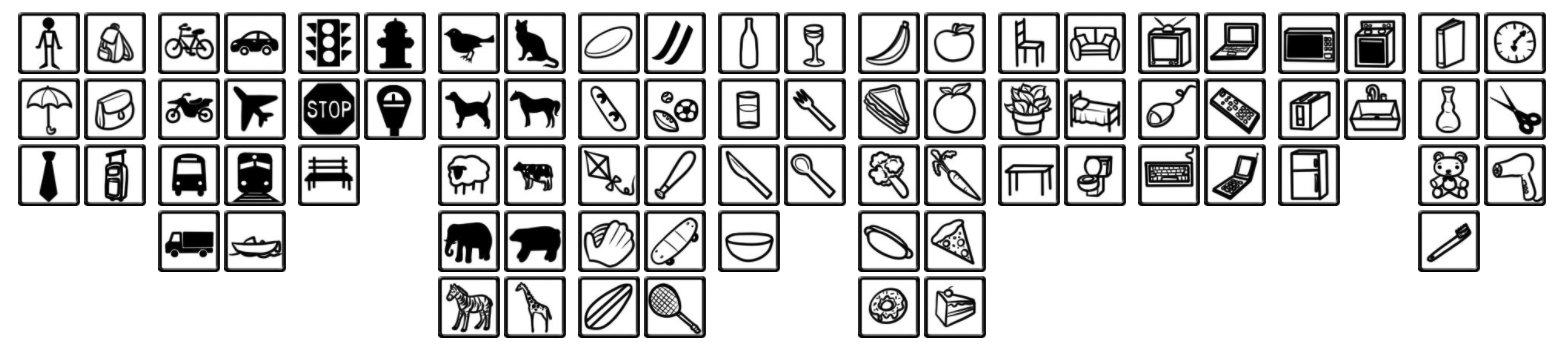
\includegraphics[width=0.9\textwidth]{img/chapters/resultados/bases-datos/cocodataset.png}
\caption{\label{fig:cocodataset}Categorías de objetos del dataset COCO}
\end{figure}

\subsection{Métricas de calidad}
\label{subsec:metricas-calidad}

\subsection{Estrategia y metodología de experimentación}
\label{subsec:estrategia-metodologia}

\section{Resultados experimentales}
\label{sec:resultados-experimentales}

\section{Conclusiones}
\label{sec:conclu-resultados}